\documentclass[../Bachelorarbeit.tex]{subfiles}

\begin{document}
\label{sec:EFT}

\begin{figure}[h]
    \centering
    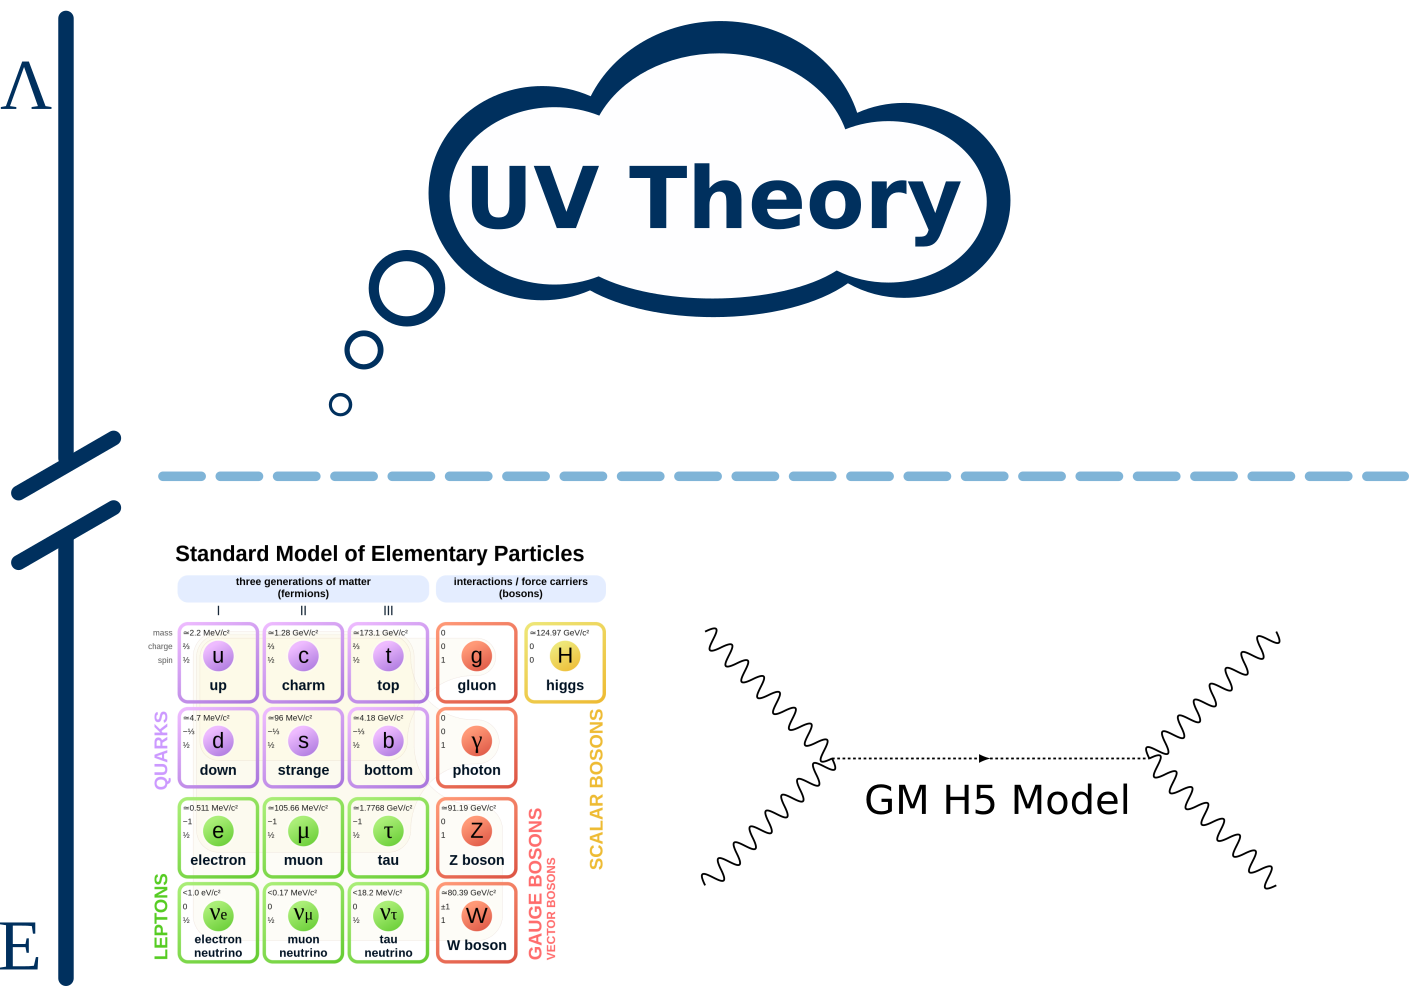
\includegraphics[width=\textwidth]{images/EFT_Model.png}
    \label{fig:EFT_sketch}
    \caption{Source and text}
\end{figure}

With the Standard Model Physicist try to describe the elementary Particles and interactions. It is successful in describing most processes in Biology, Chemistry, and Physics.
But the Standard Model is still incomplete. It can't describe Phenomenons like Gravity, Neutrino Masses, Matter-Antimatter asymmetry etc. This is where effective field theory comes in.
Here we look at the Standard Model as a low energy approximation of an underlying Ultraviolet Theory (figure~\ref{fig:EFT_sketch}). 
\\\\
It is not necessary for the purpose of this Thesis to derive Effective Field Theory(EFT) or look at complex topics like renormalization. But rather look at the Lagrangian of EFT with the Standard Model and its symmetries.
where we will also find the Dim-8 Operators. For a more rigorous derivative see~\ref{Pinco}.

\begin{equation}
    \mathcal{L}_{SMEFT} = \mathcal{L}_{SM} + \frac{1}{\Lambda} \mathcal{L}_{5} + \frac{1}{\Lambda^2} \mathcal{L}_{6} + \frac{1}{\Lambda^3} \mathcal{L}_{7} + \frac{1}{\Lambda^4} \mathcal{L}_{8} + ...
\end{equation}



\end{document}
